
\documentclass[12pt, a4paper]{article} 
\usepackage{eurosym}
\usepackage[margin = 1in]{geometry}
\usepackage[french]{babel}
\usepackage[utf8x]{inputenc}
\usepackage{graphicx}
\usepackage[T1]{fontenc}
\usepackage{fancyhdr}
\usepackage{hyperref}
\usepackage{listings}
\pagestyle{fancy}
\setlength{\headheight}{15pt}
\fancyhead[L]{SharpBoy}
\fancyhead[R]{EPITA}
\fancyhead[C]{S\_Society}
\renewcommand{\footrulewidth}{1pt} 
\fancyfoot[L]{Rapport de soutenance 2}
\fancyfoot[R]{2016-2017}
\fancyfoot[C]{\thepage}
\title{\Huge \bf SharpBoy}
\author{\LARGE \bf S\_Society }
\title{\Large \bf Rapport de Soutenance 2}


\begin{document}


\maketitle


\bigskip
\large Gabriel DUQUE: duque\_g

\bigskip
\large Antoine MARTIN: ma\_9

\bigskip
\large Martin MEUNIER : meunie\_o

\bigskip
\large Ilyes NOUMRI : noumri\_i

\bigskip
\large {\textbf{Projet S2\#}}

\bigskip 
\bigskip
\bigskip



\begin{center}
\includegraphics[width= 12cm]{logo-epita-hd.png} 
\end{center}


\pagebreak

\tableofcontents 

\pagebreak

\lstset{language=Caml}

\large
\section{Introduction}
Grâce a notre travail acharné, nous avons présenté avec plaisir notre émulateur de Chip-8 lors de la première soutenance en novembre 2016. Nous avons bien réussi la Chip-8 et cela nous a permis d'en apprendre beaucoup sur l'émulation en général.

C'est pourquoi nous nous sommes lancés sur l'émulation de la GameBoy juste après. Grâce à ces connaissances nous avons réussi à créer notre premier émulateur de GameBoy : SharpBoy, dont nous sommes tous très fiers !

Juste après notre première soutenance, nous nous sommes vite mis au travail. Ce travail comportait beaucoup de recherches sur le fonctionnement de la GameBoy et nous avions aussi beaucoup de questions sur le langage car même si nous avons beaucoup appris sur le F\#, il nous reste encore beaucoup de choses à apprendre pour factoriser et aussi améliorer notre code.

\pagebreak

\section{Retour sur le cahier des charges}
\subsection{Équipe}
L'équipe n'a pas changé et est toujours aussi motivé pour mener le projet à bien. Elle est constituée de Gabriel DUQUE, Antoine MARTIN, Martin MEUNIER, Ilyes NOUMRI.


\bigskip
\subsection{Répartition des tâches}
\bigskip

La répartition des tâches n'a pas changée même si elle reste éphémère pour la SharpBoy sachant que nous avançons beaucoup en groupe.
\bigskip


\begin{center}
\begin{tabular}{|l|c|c|c|c|}
\hline
\bf Tâches                & \bf Gabriel   & \bf Antoine   & \bf Martin    & \bf Ilyes\\
\hline 
Menus/Options       &      x       &               &         x     &       \\
\hline 
Site web            &               &         x     &               &     x  \\
\hline 
Vidéo               &          x    &               &       x       &       \\
\hline 
CPU                 & x             & x             &               &       \\
\hline 
Mémoire             &               & x             &               &  x \\
\hline
Audio               &               &               & x             & x \\
\hline
Marketing           & x             &               &               & x \\
\hline
Réseau              &               &               & x             & x \\ 
\hline
\end{tabular}
\end{center}
\bigskip
\pagebreak

\section{Avancement du projet}

\subsection{Notre émulateur de GameBoy: SharpBoy}
Actuellement, notre émulateur de GameBoy est compatible avec la ROM TETRIS. SharpBoy ne gère pas du tout les sorties audio.

Nous avons choisi de faire ceci car le son est une des parties les plus complexes de l'émulation et il n'est pas essentiel pour la majorité des jeux.

\subsection{\large Un dépôt GitHub }

Nous avons toujours notre GitHub à disposition nous permettant de travailler efficacement en groupe et de répertorier tout notre travail.

Notre organisation GitHub s-society a maintenant deux dépôts GitHub, le premier pour la Chip-8 et le deuxième, SharpBoy pour notre émulateur de GameBoy.

Nous avons encore bloqué les ajouts sur la branche principale de notre dépôt pour nous forcer à lire le code des autres avant de l'ajouter définitevement pour vérifier que tout le monde comprends bien.


\subsection{Un site Web}

Notre site Web : www.sharpboy.xyz

Ce site contient les dernières versions de notre émulateur et l'avancement de notre projet. Nous avons automatisé l'ajout d'une section commentaires à chaque article du site.

\bigskip
\section{Planning}
\begin{center}
\begin{tabular}{|l|c|c|c|}
\hline
\bf Tâches          & \bf Soutenance 2      & \bf Soutenance 3  \\
\hline 
Menus/Options       &        20\%           & 100\%  \\
\hline 
Site web            &        100\%         & 100\%  \\
\hline 
Vidéo               &        100\%          & 100\%  \\
\hline 
CPU                 &        66\%          & 100\%  \\
\hline 
Mémoire             &        66\%         & 100\%  \\
\hline
Audio               &        0\%           & 100\%  \\
\hline
Réseau              &        0\%           & 100\%  \\

\hline
\end{tabular}
\end{center}
\pagebreak
\section{Problèmes rencontrés pendant le projet}

Depuis le début du projet, nous avons rencontrés quelques soucis tout au long de la conception et l'élaboration de nos deux émulateurs.

\bigskip
En effet, lors de l'élaboration de notre Chip-8 nous avions eu des problèmes lors des phases de tests de ROMs où certains jeux ne fonctionnaient pas et nous avions du débugger notre émulateur pour trouver les problèmes. Finalement, notre émulateur de Chip-8 fonctionnait avec toutes nos ROMs.

\bigskip
Pour notre émulateur de GameBoy, SharpBoy, nous avons tout de suite vu la difficulté d'optimisation pour tous les types de ROMs existants. Il existe en effet environ 6 types de cartouches, chacune ayant une manière différente de se charger en mémoire. 

Pour faire face à ce problème, nous avons décidé de ne nous occuper que du premier type de cartouche, se chargeant en mémoire directement (les autres types sont découpés en plusieurs secteurs) pour prouver que notre émulateur fonctionne correctement car sa création n'a pas été facile. 

\bigskip
Nous avons étudié avec précision toute la documentation de l'émulation de la GameBoy qui n'était pas facile à comprendre mais que nous avons tous apprivoisée avec le temps pour être prêts sur le sujet. De plus, le son est aussi auxiliaire et nous poserait trop de problèmes à l'heure actuelle pour que nous nous en occupions.


\pagebreak

\section{Tâches à effectuer pour la dernière soutenance}

Pour notre dernière soutenance, nous prévoyons d'avoir un émulateur gérant plusieurs types de cartouches pour grandement étendre le nombre de ROMs compatibles et améliorer l'expérience de l'utilisateur.

\bigskip
Nous tenterons d'ajouter le support du son, cependant cela semble assez complexe.

\bigskip
Des ROMs comme Pokémon Rouge/Bleu devront fonctionner de manière jouable. De plus, notre émulateur comprendra plusieurs fonctionnalités utilisateur : par exemple, la prise en charge de la sauvegarde, la prise de capture d'écran, ainsi qu'une fonction Pause.


\bigskip
\begin{center}
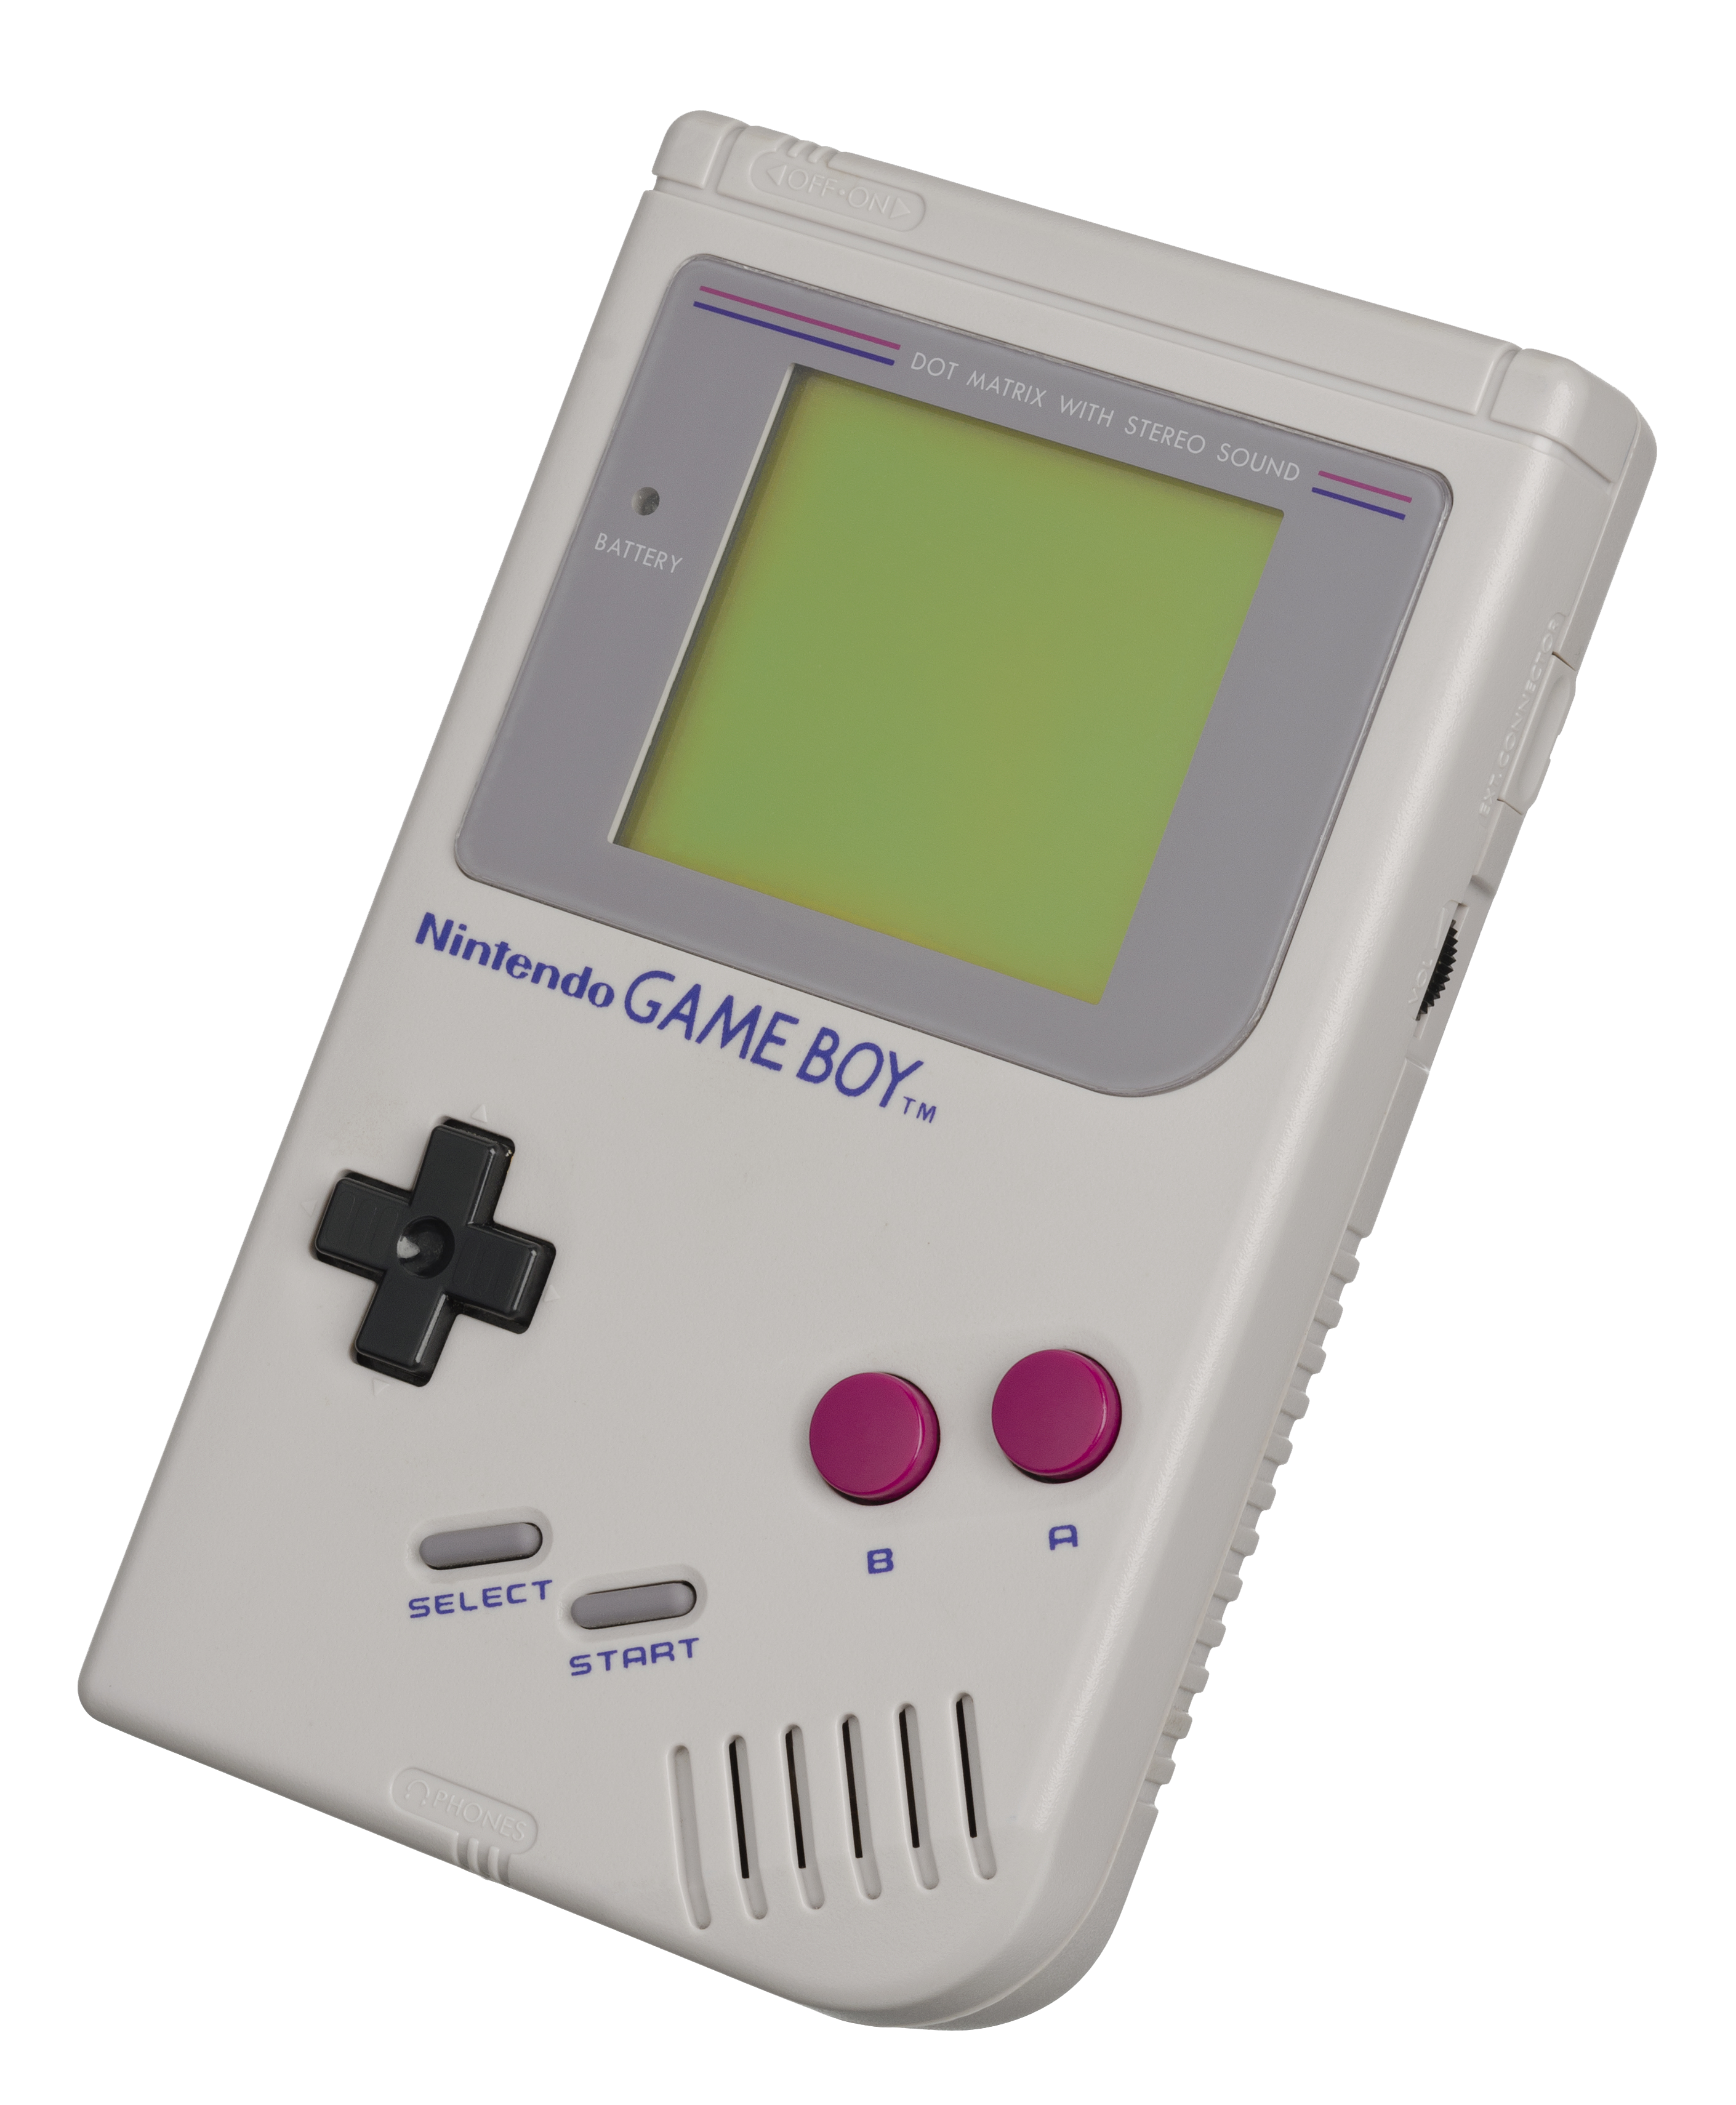
\includegraphics[width= 11cm]{Game-Boy-FL.png}
\end{center}

\pagebreak

\section{Explications techniques de notre émulateur}

\subsection{Les registres}
\small \begin{lstlisting}[frame=single]
let mutable A = 0x01uy
let mutable B = 0uy
let mutable C = 0x13uy
let mutable D = 0uy
let mutable E = 0xD8uy
let mutable F = 0b10110000uy
let mutable H = 0x01uy
let mutable L = 0x4Duy
let mutable SP = 0xFFFEus
let mutable PC = 0x0100us
\end{lstlisting}
\large
\bigskip
Ces variables représentent les registres du processeur. Les registres représentent la mémoire interne du processeur. Il s'agit de la mémoire la plus rapide d'une machine et permet de stocker les donées nécessaires à l'execution des instructions.

A part les registres SP et PC qui ont une taille de 16 bits, les registres de la GameBoy ont une taille de 8bits et certains d'entre eux peuvent combinés comme par exemple H et L pour former un registre HL de 16 bits.Dans le cas d'une juxtaposition de deux registres quatre combinaisons sont possibles: AF, BC, DE et HL. 

Certains registres sont généraux et d'autres ont une fonction qui sort du lot. Par exemple, les registres SP et PC ont une fonction particulière. En effet, le registre SP (Stack Pointer) pointe les objets les plus récemment utilisés, ceux-ci pouvant être des variables, ou des sous-fonctions. Aussi, le registre PC (Program Counter) est essentiel au fonctionnement de la GameBoy. Le program counter a pour rôle de pointer vers l'adresse de la prochaine instruction à traiter.

Le registre F est unique aussi dans son utilisation et dans ce qu'il représente mais cela sera détaillé ci-après.

\pagebreak
\subsection{Le registre F}

Le registre F est différents des autres registres mémoires :

\bigskip
Il n'est pas accessible directement au programmeur, et est modifié par les instructions exécutées. En effet, les 4 bits de poids fort sont des flags, utilisés pour marquer des évènements spécifiques survenus lors d'une instruction :

\bigskip

\begin{center}
\includegraphics{Fregister.png}
\end{center}

\bigskip
\begin{itemize}
\item Le flag Z marque si le résultat d'une opération était zéro
\bigskip
\item Le flag N marque si une soustraction a eu lieu dans une opération
\bigskip
\item Le flag H (Half Carry) marque si une opération provoque le dépassement du nombre maximum exprimable par les 4 bits de poids faible d'un registre. (Ex : 01001111 + 1 devient 01010000)
\bigskip
\item Le flag C (Carry) marque si une opération provoque le dépassement du nombre maximum exprimable par un byte (Ex : 11111111 + 1 repasse à 00000000)
\end{itemize}

\pagebreak

\subsection{Instruction DAA : Traduction binaire/décimal}

L'instruction DAA (Decimal Adjust register A) permet de convertir le contenu du registre A en code BCD (binary coded decimal).

\bigskip
Cette fonction est essentielle, elle permet en effet de traduire tous les chiffres que la ROM veut afficher du binaire vers le décimal, permettant un affichage lisible "humainement" pour l'utilisateur.

\bigskip

\small{\begin{lstlisting}[frame=single]
let daa () =
    let lowBCD = A % 10uy
    let highBCD = ((A % 100uy) - lowBCD) / 10uy
    let result = (highBCD <<< 4) ||| lowBCD
    ZF <- (result = 0uy)
    HF <- false
    CF <- A >= 100uy
    A <- result
\end{lstlisting}}

\bigskip
\large

Note : l'ajout de parenthèses vides après le nom de la fonction dans la déclaration permet au compilateur de la distinguer d'une variable, et donc de ne pas l'évaluer lorsqu'elle est déclarée mais lorsqu'elle sera appelée.

\bigskip
La fonction, une fois son but effectué, modifie plusieurs flags du registre F pour indiquer le résultat de l'opération :

\bigskip
\begin{itemize}
\item Le flag C indique si une conversion vers du code BCD a bien été effectuée
\item Le flag H est remis à 0 lors de l'exécution de cette opération
\item Le flag Z indique si A vaut maintenant 0
\end{itemize}

\pagebreak
\subsection{La fonction Draw}
\small \begin{lstlisting}[frame=single]
let Draw (args:PaintEventArgs) =
  for y in [0..HEIGHT-1] do
    for x in [0..WIDTH-1] do
      args.Graphics.FillRectangle(brushes.[screen.[(y*WIDTH) + x]],
      x * SCALE, y * SCALE, SCALE, SCALE)
\end{lstlisting}
\large
La fonction Draw est une fonction utilisant System.Drawing et Windows.Form qui permet de dessiner sur l'écran de la GameBoy grâce à deux boucles permettant de parcourir tout l'écran. La fonction dessine grâce à FillRectangle qui reçois les coordonnées du rectangle à remplir.

\bigskip

\subsection{Exemple de fonctions d'incrémentations}
\small { \begin{lstlisting}[frame = single]
let inc (reg:byte byref) =
     reg <- reg + 1uy
     ZF <- (reg = 0uy) 
     NF <- false
     HF <- (reg = 0xF0uy)
     
let incHL () =
    temp <- readAddress_2(H,L)
    inc(&temp) 
    writeAddress_2(H,L,temp)

let incrementHL(inc:bool) =
     temp16 <- uint16 H <<< 8 ||| uint16 L 
     (if inc then temp16 <- temp16 + 1us else temp16 <- temp16 - 1us) 
     H <- byte ((temp16 &&& 0xFF00us) >>> 8) 
     L <- byte (temp16 &&& 0x00FFus)
\end{lstlisting}} 
\bigskip

\large
La fonction inc permet d'incrémenter la variable contenue dans les registre donné en argument, ainsi que définir la valeur des flags ZF, NF et HF. 
Les fonctions incHL et incrementHL sont utilisées dans des instructions.
incHL permet d'incrémenter la valeur dans l' adresse du registre HL . Le mot clé \& indique que l'on veut passer une variable par référence. incrementHL, quant à elle, permet d'incrémenter l'adresse du registre HL si le booléen est à true sinon il la décrémentera.

\pagebreak

\section{Conclusion}
Ce projet nous a permis d'améliorer nos compétences en F\# et nos connaissances dans l'émulation en général.

\bigskip
Avoir un émulateur fonctionnel, pouvant être utilisé pour jouer à quelques ROMs est pour nous une belle victoire, et nous avons appris énormément de choses en le réalisant.

\bigskip
Nous espérons avoir un émulateur qui puisse démarrer des ROMs plus complexes et ayant de nouvelles fonctionnalités d'ici la soutenance finale.

\bigskip 
L'implémentation du son sera sûrement le plus grand défi, avec le chargement des ROMs au format de cartouche différent.

\bigskip
In fine, le projet nous permet de progresser en programmation d'une manière plutôt intéressante dans le sens où, indépendamment du fait d'apprendre une nouveau langage, nous avons pu comprendre et assimiler des notions assez complexes concernant l'algorithmique en général et l'architecture des systèmes.


\pagebreak
\section{Bibliographie}
MSDN - Pour la documentation du F\#:

\url{https://msdn.microsoft.com/en-us/visualfsharpdocs/}

\url{conceptual/visual-fsharp-development-portal}

\bigskip
FSharp.org - Pour l'apprentissage du F\#:

\url{http://fsharp.org/}

\bigskip
FSharp For Fun and Profit:

\url{http://fsharpforfunandprofit.com}

\bigskip

Page Wikipedia de la GameBoy:

\url{https://en.wikipedia.org/wiki/Game_Boy}

\bigskip

Documentation technique de la GameBoy:

\url{http://marc.rawer.de/Gameboy/Docs/GBCPUman.pdf}

\bigskip
Tableau des instructions pour la GameBoy:

\url{http://pastraiser.com/cpu/gameboy/gameboy\_opcodes.html}

\pagebreak
\section{Captures d'écrans}

\begin{center}
\includegraphics[width= 11cm]{Capture1.PNG}
\end{center}

\bigskip

\begin{center}
\includegraphics[width= 11cm]{Capture3.PNG}
\end{center}
\pagebreak

\center{\includegraphics[width=11cm]{brickbreaker}}


\bigskip

\center{\includegraphics[width=11cm]{drmario.jpg}}





\end{document}
